%File: claimarc_aaai.tex
\documentclass[letterpaper]{article}
\usepackage[submission]{aaai2026}
\usepackage{times}
\usepackage{helvet}
\usepackage{courier}
\usepackage[hyphens]{url}
\usepackage{graphicx}
\urlstyle{rm}
\def\UrlFont{\rm}
\usepackage{natbib}
\usepackage{caption}
\usepackage{amsmath,amssymb}
\usepackage{booktabs}
\usepackage{multirow}
\usepackage{array}
\frenchspacing
\setlength{\pdfpagewidth}{8.5in}
\setlength{\pdfpageheight}{11in}
\pdfinfo{/TemplateVersion (2026.1)}
\setcounter{secnumdepth}{0}

\newcommand{\best}[1]{\textbf{#1}}
\newcommand{\std}[1]{{\scriptsize$\pm$#1}}

\title{Detecting Consumer-Perceived Deception in Livestream Commerce: A Retrieval-Augmented Contrastive Learning Approach}
\author{Anonymous Submission}
\affiliations{}

\begin{document}
\maketitle

\begin{abstract}
The high conversion of livestream commerce rests on a streamer's real-time pitch, and the exaggerated promises, implicit assurances, and selective emphasis made to close a sale create a risk that buyers feel misled once the product arrives---a risk to brand trust and to platform compliance. We study this risk at the level of individual product attributes, jointly modeling the tension between what a streamer claims and what the product is, and casting consumer-perceived deception as a binary target supported by post-purchase reviews, with each label carrying a weight that reflects how strongly the reviews support it. Our model, CLAIMARC, encodes the claim and the product evidence as two streams over a shared retrieval backbone, keeps them comparable at the token level through bidirectional cross-attention, and adds to cross-entropy a retrieval-augmented contrastive objective that tightens same-label neighborhoods and separates semantically close opposite-label ones---giving the model traction on borderline pairs where similar wording flips the perceived label. The design also offers a deployment benefit: once trained, the encoder is fixed, and new streamers, categories, and risk phrases are absorbed by maintaining an external retrieval index. On a self-built Chinese corpus of 4{,}883 attribute-level pairs, CLAIMARC reaches 82.6 accuracy, 73.4 positive-class F1, 75.4 average precision (AP), and 90.4 AUC, ahead of same-backbone baselines and zero-shot, few-shot, and fine-tuned large-language-model systems; geometry, cross-domain, and selective-prediction analyses trace the advantage to the learned retrieval geometry rather than the retrieval rule. The framework offers platforms an interpretable, auditable risk signal and gives merchants early warning of phrasing likely to trigger post-purchase complaints.
\end{abstract}

\section{Introduction}

Livestream e-commerce has become one of the central channels of online retail in China, where annual gross merchandise value exceeds RMB 4.5 trillion---about a third of online retail---and contributes most of the sector's growth. The rapid expansion is accompanied by a parallel rise in consumer complaints and regulatory penalties: recent Chinese rules list exaggerated claims, fabricated usage effects, and the selective omission of key information as priority targets and require platforms to build real-time monitoring and disposal mechanisms over the livestream process itself \citep{samr2025livestream}. Misleading advertising produced while a streamer presents a product has thus turned into a systemic compliance risk that simultaneously threatens consumer rights, brand trust, and platform governance.

A platform's first need is to flag, automatically and at scale, where a streamer's description diverges from the product. This is harder than it sounds. Livestreaming is an intensely persuasive medium of multi-turn narration, live demonstration, and constant interaction, in which neutral description, emotive promotion, and comparison are interleaved and expectations are shaped as much by pace, tone, and repetition as by content. Whether a passage misleads is decided not by any one sentence but by how the claim sits against the product facts and by how consumers read it. Three properties of this setting set it apart from fact verification or rumor detection.

\textbf{The supervision anchor shifts.} NLP veracity research---NLI-style fact verification \citep{thorne2018fever}, open-domain verification \citep{guo2022survey}, and retrieval-augmented LLM systems \citep{putta2025claimcheck}---assumes that falsehood is a verifiable contradiction between statement and fact. The risk a platform bears, however, is whether buyers feel misled, which often diverges from objective inconsistency. A claim may stray from the facts yet sit off the path of buyer expectations and carry little risk; a literally accurate claim may, through selective emphasis, comparison, repetition, or persona-backed endorsement, open a gap that buyers feel only once the product arrives. What matters is credibility, not veracity \citep{mavlanova2012signaling}. Supervision must therefore come from consumer reviews---self-selected \citep{li2008selfselection}, negatively skewed \citep{baumeister2001bad}, and vulnerable to manipulation \citep{mayzlin2014promotional,luca2016fake,he2022fakemarket}---and reviews become usable labels only with explicit reliability modeling. Because complaints attach to specific attributes, the unit of judgment is the product attribute rather than the whole passage.

\textbf{The hard cases live inside a single attribute.} Pairs that consumers label oppositely tend to share wording and facts and to differ only in degree: the same shirt is ``comfortable'' in one stream and ``so comfortable you'll never take it off'' in another; individually true points about fabric, make, and price are assembled into an unwarranted ``counter-grade'' positioning; a limitation that matters to the purchase is simply left unsaid. The discriminative signal thus lies between near-identical, oppositely labeled examples \emph{within} an attribute, not across categories or styles---exactly where models that pool same-attribute pairs into one neighborhood, zero-shot LLMs included, tend to fail.

\textbf{The distribution moves, and deployment must keep up.} Streamers, categories, and risk phrases turn over weekly, and retraining a large model at each shift is impractical. A more sustainable design pushes the adjustable part of the decision out of the weights and into an external library: once the representation encodes the task's geometry, new labeled cases extend coverage by being indexed rather than re-learned \citep{mei2024rgcl,mei2025rahmd}. Retrieval-based moderation has shown such robustness over parametric classifiers \citep{wang2025moderation,long2023retrievalicl}, but it leaves open how a representation should carry the perception axis and how its hard negatives should align with that boundary.

CLAIMARC---a \emph{Claim-Aware Misleading-Advertising} detector with \emph{Retrieval-augmented Contrastive} learning---addresses these requirements as one pipeline. It works at the attribute level: streamer claims about an attribute are gathered on one side, and structured parameters, detail-image text, and visual cues are assembled as evidence on the other, while aligned post-purchase reviews give a binary perception label and its reliability weight. A shared retrieval encoder reads the two sides as parallel streams and lets them rewrite each other through bidirectional cross-attention, keeping claim and fact comparable at the token level; the fused state feeds both a perceived-risk classifier and a retrieval embedding. The embedding is trained with a reliability-weighted, class-balanced contrastive loss that draws each example toward same-label neighbors and away from semantically close opposite-label ones, so that look-alike pairs with opposite perceived labels are separated. At deployment the encoder is fixed, and new streamers or risk phrases are absorbed by writing their labeled cases into the retrieval index, with a vote--classifier agreement check routing uncertain cases to human review.

This work makes three contributions. First, we recast livestream misleading-advertising detection as attribute-level consumer-perception discrimination, building a computable target with a per-instance reliability weight from reviews and connecting the marketing account of perceived deception to a scalable detector. Second, we present CLAIMARC, which couples dual-stream claim--evidence comparison with retrieval-augmented contrastive learning tailored to noisy, review-derived labels. Third, through controlled baselines, representation geometry, cross-domain transfer, ablations, and selective prediction, we show that the gain comes from the learned representation rather than the retrieval rule, and that the fixed encoder adapts to unseen streamers through index maintenance alone.

\section{Related Work}

\textbf{Persuasive communication and misleading risk in livestream e-commerce.} Most research on persuasion and purchase in livestreaming starts from the consumer side, characterizing how streamer traits, social presence, and interaction mechanisms shape trust and purchase intention \citep{wongkitrungrueng2020livestream,sun2019livestream,park2020internetcelebrity}. In this anthropomorphic, strongly situated channel, cognitive and affective trust in the streamer act on purchase decisions beyond the product itself, and the streamer's professional persona, interaction warmth, and emotional intensity are repeatedly identified as key antecedents \citep{lu2021livestream,hu2020livestream}. From a signaling view, the streamer is a far more persuasive signal source than static website cues, so signal credibility rather than objective veracity governs the mitigation of information asymmetry \citep{mavlanova2012signaling}. Regulators have meanwhile listed exaggerated claims, fabricated usage effects, and selective omission as compliance priorities \citep{samr2025livestream}. These works ground the phenomenon at the level of streamer strategy or platform governance, but do not provide an operational way to decide, at industrial scale, which utterance, on which attribute, poses a misleading risk to consumers. The construct closest to ours is perceived deception: marketing research argues that once consumers perceive deception, negative evaluations extend to the whole category and even unrelated brands \citep{agakhani2019brand}, and that perceived deception mediates repurchase and e-WOM in online retail \citep{riquelme2014perceived}. This literature, mostly survey- or experiment-based, has not been connected to a deployable automatic detector or grounded in the concrete contrast between streamer claims and product facts. CLAIMARC operationalizes the construct with review-aligned labels.

\textbf{Automated fact verification and claim-evidence representation learning.} Fact verification is the line most directly aligned with veracity judgment. \citet{vlachos2014factchecking} formalized it as a claim-extraction, evidence-retrieval, and verdict pipeline; FEVER standardized a Wikipedia-grounded support/refute/not-enough-info task and spurred a series of NLI-based discriminators \citep{thorne2018fever,bowman2015snli}. Later work extended evidence granularity and robustness: MultiFC moved to multiple domains \citep{augenstein2019multifc}, SciFact to scientific literature \citep{wadden2020scifact}, and VitaminC stressed genuine sensitivity to evidence rather than lexical shortcuts \citep{schuster2021vitaminc}; \citet{guo2022survey} survey the field. Claim-evidence interaction modeling is the most method-relevant strand: ESIM established the standard local alignment-and-composition design \citep{chen2017esim}, and pretrained encoders since BERT fold such interaction into self-attention with $[\mathrm{CLS}]$ pooling \citep{devlin2019bert,cui2021wwm}. For sarcasm-cause identification, \citet{li2025sarcasm} combine dual-stream self-attention with cross-stream attention and outperform single-stream concatenation, dual-encoder cosine, and ESIM, showing that when the task is a fine-grained contrast between two streams, token-level cross-attention preserves structure that pooling discards. Retrieval-augmented LLMs form another recent route that feeds external evidence into the pipeline \citep{putta2025claimcheck,vladika2024survey}, mainly addressing knowledge freshness while relying on autoregressive reasoning. This line mismatches our task in three ways: it assumes an objective truth set, whereas our target is a subjective post-purchase deviation anchored in reviews; its boundary cases are lexical-overlap-with-reversed-relation, whereas ours include expressive strength, combinatorial misleading, selective salience, and stylized endorsement; and its judgments are passage-level, whereas consumer complaints are almost always attribute-specific.

\textbf{Consumer reviews as construct measurement signals.} Reviews have long served as research signals across information systems, marketing, and NLP. Since \citet{hu2004mining}, aspect-based sentiment analysis has become the standard way to structure reviews into attribute-level signals \citep{pang2008opinion,liu2012sentiment}; weak supervision reduces annotation cost further \citep{angelidis2018aspect,karamanolakis2019keyword}. Reviews are nonetheless non-uniform: early reviewers self-select and polarize \citep{li2008selfselection}, negative information is more diagnostic than positive \citep{baumeister2001bad,chevalier2006wom}, and reviews face authenticity problems---platform entry constraints affect promotional fake-review density \citep{mayzlin2014promotional}, competitive pressure drives manipulation \citep{luca2016fake}, and a market for fake reviews exists \citep{he2022fakemarket}. Methods that detect fake reviews target review forgery itself \citep{jindal2008spam,mukherjee2013yelp}. In our setting the question is not to filter each review but to assess how far an attribute-level label is supported by trustworthy reviews---a measurement-reliability problem. The Dawid--Skene multi-rater model provides a classic framework for such heterogeneous reliability \citep{dawid1979em}, whose reliability-weighting spirit continues in modern weak supervision \citep{ratner2017snorkel}. We therefore construct attribute-level supervision at the intersection of structured aggregation and authenticity, carried by a per-sample reliability weight.

\textbf{Retrieval-augmented contrastive learning and dynamic adaptation.} Supervised contrastive learning shapes geometry by class \citep{khosla2020supcon}, with repeatable advantages over cross-entropy in robustness and geometry quality \citep{graf2021dissecting}. Hard-negative selection is a key variable: hardness-tilted sampling in self-supervision \citep{robinson2020hardneg}, hardness in supervised contrast \citep{jiang2022hscl}, and momentum-based, label-aware hard negatives that improve in- and cross-domain hate-speech detection \citep{kim2024lahn} together show that contrastive discriminability depends on whether negatives lie near the target boundary, not on their count. Coupling retrieval with contrast is most directly related: dense passage retrieval made contrastive learning the standard for retrieval representations \citep{karpukhin2020dpr}, and SimCSE and retrieval-pretrained backbones (including the BGE family we use) let a shared backbone serve both understanding and neighbor retrieval \citep{gao2021simcse,xiao2023cpack}. RGCL retrieves hard negatives by periodically rebuilding a FAISS index so the geometry separates confounders \citep{mei2024rgcl}, extended to large multimodal models in RA-HMD \citep{mei2025rahmd}; in moderation, embedding-retrieval systems show adaptation advantages over parametric classifiers \citep{wang2025moderation,long2023retrievalicl,johnson2019faiss}. Once the geometry is encoded, absorbing a new distribution becomes index extension rather than retraining, with both parametric and neighbor judgments available at inference \citep{wang2020alignment}. CLAIMARC adapts this line to consumer-perception labels: it mines class-balanced, reliability-weighted positives and hard negatives so that the contrast concentrates on look-alike pairs with opposite labels, the region where the perception boundary actually lies.

\section{Task and Data}

For a product $p$ in category $c(p)$, let $T_p$ be the stream transcript, $F_p$ the product-side fact sources, and $R_p$ the post-purchase reviews. Each category has a normalized attribute schema $A_c$. An instance is a pair $(p,a)$, where $a \in A_{c(p)}$ is an attribute mentioned by reviews or recovered as an objective-negative claim attribute. The model observes a claim passage $X^c_{p,a}$ extracted from $T_p$ and an evidence passage $X^e_{p,a}$ assembled from structured parameters, detail-image OCR, and visual-language observations. The target $y_{p,a}\in\{0,1\}$ denotes whether consumers perceive the streamer's claim about $a$ as misleading. The detector learns $f:(X^c_{p,a},X^e_{p,a})\mapsto\hat y_{p,a}\in[0,1]$.

\textbf{Data construction.} The pipeline has three stages. First, product-parameter keys and review aspects are normalized into category-specific attribute schemas through embedding clustering and large-language-model adjudication. Second, schema-guided extraction identifies streamer claim spans with hard span-consistency constraints and aligns each review to the claim that discusses the same attribute. Third, product evidence is collected from structured parameters, detail-image OCR, and visual-language observations, kept as a parallel evidence list without merging. A pair is labeled positive when at least one aligned review carries negative polarity about the attribute; otherwise it is negative. We additionally mine \emph{objective-negative} pairs---attributes the streamer claimed but for which no aligned consumer complaint exists---to broaden coverage of normal promotional speech; these are weighted by evidence coverage.

\textbf{Reliability weighting.} Each instance receives $c_{p,a}\in[0,1]$, a measurement-reliability weight that multiplies the saturation of aligned-review count, alignment coverage, the asymmetric diagnosticity of negative evidence, and a discount for suspected promotional or low-diversity reviews. The weight is lower-bounded at $0.05$ to retain weak supervision while preventing thin or suspicious evidence from dominating training; it is used as a per-sample multiplier in both the cross-entropy and the contrastive loss.

\textbf{Corpus.} The final corpus contains 4{,}883 product-attribute pairs from Chinese livestream sessions collected between October 2024 and March 2025, covering 10 first-level categories, 38 sub-categories, 108 rooms, and 1{,}532 normalized attributes. Of the pairs, 2{,}278 are review-driven and 2{,}605 are objective-negative; the positive class is 25.6\%. We split by room ID at a 70:10:20 ratio so that all pairs from one room fall in a single split, eliminating streamer leakage (Table~\ref{tab:data}).

\begin{table}[t]
\centering\small
\setlength{\tabcolsep}{8pt}
\begin{tabular}{lrrr}
\toprule
Split & \#Pairs & Pos.\% & \#Rooms \\
\midrule
Train & 3{,}636 & 24.2 & 92 \\
Validation & 392 & 31.1 & 5 \\
Test & 855 & 29.1 & 11 \\
\midrule
All & \best{4{,}883} & \best{25.6} & \best{108} \\
\bottomrule
\end{tabular}
\caption{Room-grouped partition. Review-driven pairs: 2{,}278; objective-negative pairs: 2{,}605. Evidence-source coverage (0/1/2/3): 1{,}483/1{,}826/1{,}118/456 (mean 1.11). Reliability weight $c$: mean 0.46, median 0.48.}
\label{tab:data}
\end{table}

\section{CLAIMARC}

\textbf{Dual-stream input.} For each $(p,a)$, CLAIMARC builds two sequences. The claim flow begins with an attribute anchor and the normalized attribute name, then lists the claim spans for $a$; a null-claim placeholder is inserted when the streamer made no claim about $a$. The evidence flow begins with the same attribute anchor, then lists product-side evidence grouped by source (parameters, OCR text, visual-language observations). Both flows are truncated to 384 tokens, with priority given to direct product parameters.

\textbf{Shared encoder and fusion.} A single BGE-large-zh-v1.5 encoder \citep{xiao2023cpack} processes both streams and is trained end to end with the fusion module and the heads. Sharing the backbone places the queries and keys of cross-attention on one manifold, so attention scores read as claim--evidence alignment. The encoded states pass through $N{=}2$ TwoStreamFusion blocks; each applies intra-stream self-attention, bidirectional cross-attention with projections shared across the two directions, and a SwiGLU feed-forward network, in a pre-LayerNorm arrangement \citep{li2025sarcasm}. Let $\bar h_c$ and $\bar h_e$ be the final CLS states.

\textbf{Classifier and retrieval heads.} The forward classifier uses the ESIM-style pair representation \citep{chen2017esim}
\begin{equation}
z=[\bar h_c;\bar h_e;\bar h_c-\bar h_e;\bar h_c\odot \bar h_e],
\end{equation}
followed by layer normalization and a linear sigmoid head, trained with reliability-weighted binary cross-entropy
\begin{equation}
\mathcal{L}_{\mathrm{CE}}=-\sum_i c_i\big[y_i\log\hat y_i+(1-y_i)\log(1-\hat y_i)\big].
\end{equation}
The retrieval head maps the same comparison representation to a 256-dimensional unit vector $g_{p,a}$.

\textbf{Retrieval-augmented contrast.} Training runs in two phases: three warm-up epochs with $\mathcal{L}_{\mathrm{CE}}$ alone, then six epochs that add the RACL loss. At the start of each contrastive epoch the training-set embeddings are written to a memory bank. For anchor $i$, positives $\mathcal{P}_i$ are its $K_p$ nearest same-label neighbors and hard negatives $\mathcal{N}_i$ its $K_n$ nearest opposite-label neighbors. With $s_{uv}=\exp(g_u^\top g_v/\tau)$, the loss is
\begin{equation}
\mathcal{L}_{\mathrm{CL}}=\sum_i \frac{c_i\, b_{y_i}}{|\mathcal{P}_i|}
\sum_{j\in\mathcal{P}_i}-\log\frac{s_{ij}}{s_{ij}+\sum_{k\in\mathcal{N}_i}s_{ik}},
\end{equation}
where $b_{y_i}$ is an inverse-frequency factor that keeps the minority misleading class from being swamped. The total objective is $\mathcal{L}_{\mathrm{CE}}+\lambda_{\mathrm{CL}}\mathcal{L}_{\mathrm{CL}}$. The warm-up lets the encoder settle on a stable decision boundary before the retrieval geometry is shaped on top of it.

\textbf{Inference and library use.} The main prediction uses the forward classifier. A global reliability-weighted $k$-nearest-neighbor vote over $g$,
\begin{equation}
\hat y^{\mathrm{RKC}}_t=\frac{\sum_{j\in\mathrm{kNN}(t)} c_j\cos(g_t,g_j)\,y_j}{\sum_{j\in\mathrm{kNN}(t)} c_j\cos(g_t,g_j)},
\end{equation}
serves two auxiliary roles: it lets a retrieval library absorb new labeled domains, and its disagreement with the classifier, $|\hat y_t-\hat y^{\mathrm{RKC}}_t|$, gates selective abstention.

\section{Experiments}

We address four research questions. \textbf{RQ1}: Does CLAIMARC improve in-distribution screening over fact-verification, classification, frozen-retrieval, and LLM baselines? \textbf{RQ2}: Does RACL reshape the representation toward separable consumer-risk geometry? \textbf{RQ3}: Does the model transfer to unseen categories and streamers, including gradient-free library adaptation? \textbf{RQ4}: Which components, retrieval choices, and label-construction decisions drive the result?

\textbf{Baselines.} Group~(A), \emph{objective fact verification}, bounds what is achievable when the anchor is a mechanically verifiable contradiction: ESIM \citep{chen2017esim}, decomposable attention \citep{parikh2016decomp}, and a Chinese BERT-NLI cross-encoder. Group~(B), \emph{text classification}, is closest to our method: TextCNN, BiLSTM, BERT-base-Chinese, and Chinese-RoBERTa-wwm-ext, the last two reading $[\mathrm{CLS}]\,X^c\,[\mathrm{SEP}]\,X^e\,[\mathrm{SEP}]$. Group~(C), \emph{frozen-encoder retrieval probes}, trains LR, linear SVM, MLP, or a reliability-weighted kNN vote on frozen BGE pair features, isolating what the representation already encodes before any contrastive training. Group~(D), \emph{large language models}, includes zero-shot and five-shot chain-of-thought gateway models and Qwen2.5-7B-Instruct with LoRA SFT under matched supervision.

\textbf{Metrics and implementation.} Consumer-perception screening is a class-imbalanced, ranking-oriented problem, so AP (the area under precision-recall, $=$ AUPRC) is the primary metric; we also report AUC, accuracy, and positive-class F1 at a validation-selected threshold, and estimate significance with $n{=}2{,}000$ paired bootstrap. The shared backbone is BGE-large-zh-v1.5 ($d{=}1024$), trained end to end with the fusion module and heads. TwoStreamFusion stacks two pre-LN blocks (8 heads, shared bidirectional cross-attention, SwiGLU). Training uses AdamW, encoder learning rate $10^{-5}$, head learning rate $10^{-4}$, bf16, effective batch size 36, $\lambda_{\mathrm{CL}}{=}0.5$, $\tau{=}0.07$, $K_p{=}3$, $K_n{=}5$. CLAIMARC headlines the forward classifier; the retrieval vote (RKC) is reserved for library adaptation (\S~Cross-Domain) and selective prediction (\S~Selective Prediction). All learnable systems use three seeds; leave-one-category reports mean over 10 folds.

\subsection{Main Comparison (RQ1)}

CLAIMARC leads every metric in Table~\ref{tab:main} (Acc 82.6, F1 73.4, AP 75.4, AUC 90.4), and the margins are widest on the two ranking metrics that matter for screening: at a matched end-to-end budget it improves AP over the strongest fine-tuned encoder, RoBERTa-CLS, from 69.0 to 75.4, and over BERT-CLS from 68.2. The four baseline groups each tell us why. Objective fact verification trails furthest behind---ESIM reaches only 51.2 AP and even the BERT-NLI cross-encoder stalls at 67.9---which confirms that perceived misleadingness seldom reduces to a logical contradiction with the evidence. Within the text-classification family, the from-scratch sequence models (TextCNN 60.9, BiLSTM 66.3) lag the pretrained encoders by a clear margin, so the retrieval-pretrained backbone is doing real work rather than merely adding capacity. The large language models are the most striking: in the zero- and five-shot settings their ranking collapses to chance (AP 27--29, AUC $\le0.50$), and although matched LoRA SFT recovers Qwen2.5-7B to 63.8 AP, it still trails CLAIMARC by more than ten AP points at roughly twenty times the parameters, indicating that a generic parametric prior does not encode the consumer-perception axis. Finally, the frozen-encoder probes locate the source of the gain: a frozen BGE kNN reaches only 64.4 AP and the best probe (MLP) 67.6, so the retrieval representation alone is not enough---the advantage emerges only once contrastive training reshapes the geometry. Consistent with this reading, Figure~\ref{fig:prroc} shows CLAIMARC pulling ahead precisely in the high-recall region where a screening tool operates.

\begin{table*}[t]
\centering\small
\setlength{\tabcolsep}{7pt}
\begin{tabular}{llcccc}
\toprule
Group & System & Acc & F1 & AP & AUC \\
\midrule
\multirow{3}{*}{(A) Objective fact verification}
 & ESIM & 73.8\std{0.6} & 65.9\std{2.1} & 51.2\std{1.6} & 79.9\std{1.3} \\
 & Decomposable Attention & 76.2\std{0.4} & 61.5\std{1.6} & 60.5\std{2.6} & 83.6\std{0.1} \\
 & BERT-NLI cross-encoder & 79.1\std{0.5} & 65.1\std{3.2} & 67.9\std{1.1} & 87.4\std{0.6} \\
\midrule
\multirow{4}{*}{(B) Text classification}
 & TextCNN & 76.5\std{0.8} & 57.0\std{2.6} & 60.9\std{0.9} & 84.1\std{0.8} \\
 & BiLSTM & 79.2\std{0.3} & 65.5\std{2.6} & 66.3\std{0.9} & 86.4\std{0.3} \\
 & BERT-base + [CLS] & 80.9\std{0.5} & 71.7\std{1.0} & 68.2\std{1.8} & 88.3\std{0.4} \\
 & RoBERTa-wwm + [CLS] & 80.5\std{0.8} & 70.0\std{1.8} & 69.0\std{1.0} & 88.4\std{0.1} \\
\midrule
\multirow{4}{*}{(C) Frozen-encoder retrieval probes}
 & BGE-frozen + LR & 77.0 & 68.5 & 66.4 & 86.6 \\
 & BGE-frozen + linear SVM & 76.0 & 68.0 & 60.5 & 84.8 \\
 & BGE-frozen + MLP & 78.6 & 67.4 & 67.6 & 86.4 \\
 & BGE-frozen + kNN vote & 78.1 & 62.1 & 64.4 & 83.0 \\
\midrule
\multirow{3}{*}{(D) Large language models}
 & Qwen-Flash (0-shot) & 49.8 & 30.5 & 27.4 & 46.1 \\
 & GPT-5.4 (5-shot CoT) & 58.2 & 24.8 & 26.9 & 44.6 \\
 & Qwen2.5-7B + LoRA SFT & 73.0 & 61.7 & 63.8 & 81.9 \\
\midrule
\textbf{CLAIMARC} & forward classifier (ours) & \best{82.6}\std{0.4} & \best{73.4}\std{0.5} & \best{75.4}\std{1.3} & \best{90.4}\std{0.4} \\
\bottomrule
\end{tabular}
\caption{Main comparison on the test set (\%, $N{=}855$, 249 positives). Trainable systems report mean $\pm$ s.d.\ over three seeds; frozen probes and LLMs are run once. Accuracy and F1 use a validation-selected threshold; AP and AUC are threshold-free. All gateway LLMs in zero-/five-shot score AP 27--29 and AUC $\le0.50$; representative rows are shown. Best per column in bold.}
\label{tab:main}
\end{table*}

\begin{figure}[t]
\centering
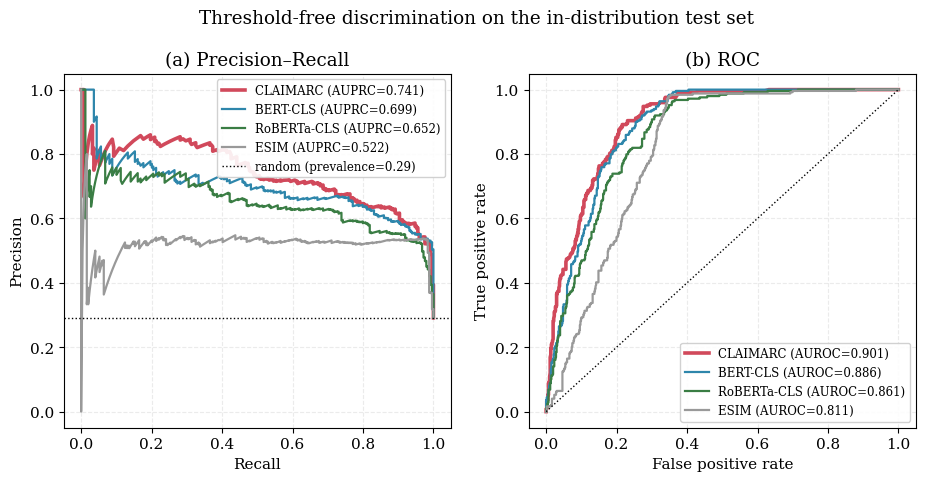
\includegraphics[width=\columnwidth]{figs/fig_pr_roc.pdf}
\caption{Threshold-free discrimination on the test set. CLAIMARC (red) leads the precision-recall curve, most visibly in the high-recall screening region, and the ROC curve. The dotted line marks the positive prevalence (0.29).}
\label{fig:prroc}
\end{figure}

\subsection{Cross-Domain Generalization (RQ3)}

A screening model is only useful if it survives the constant churn of new categories and streamers, so we next test transfer to unseen domains with no target adaptation, building CLAIMARC's retrieval library from source pairs alone (Table~\ref{tab:xdom}). When an entire category is held out (10 folds), CLAIMARC keeps the best ranking on the unseen category (AUC 90.0, AP 71.0) and, just as importantly, the tightest spread across folds (AUC s.d.\ 4.0 against BERT-CLS's 4.7), so its advantage does not hinge on which category it happens to see. Holding out twenty streamers widens the gap further (AUC 93.1, AP 81.4, about 2.5 AP over the strongest fine-tuned encoder), as one would expect when the discriminative axis is consumer perception rather than streamer identity. The language models, by contrast, remain at or below chance under both protocols (AUC $\le0.52$), reinforcing that their parametric prior carries little of this axis.

\begin{table}[t]
\centering\small
\setlength{\tabcolsep}{4pt}
\begin{tabular}{lcccc}
\toprule
& \multicolumn{2}{c}{Leave-1-category} & \multicolumn{2}{c}{Leave-20-streamers} \\
\cmidrule(lr){2-3}\cmidrule(lr){4-5}
System & AUC & AP & AUC & AP \\
\midrule
ESIM & 85.1\std{6.7} & 56.5\std{12.2} & 88.2\std{0.4} & 68.4\std{0.7} \\
BERT-CLS & 89.4\std{4.7} & 70.1\std{8.0} & 92.2\std{0.0} & 78.7\std{0.3} \\
RoBERTa-CLS & 88.5\std{4.3} & 67.3\std{6.7} & 92.0\std{0.2} & 78.9\std{0.8} \\
LLM 0-shot & 45.2\std{5.1} & 25.6\std{12.6} & 47.0\std{0.3} & 29.3\std{0.2} \\
LLM 5-shot & 45.6\std{4.5} & 25.7\std{12.1} & 52.1\std{0.8} & 32.4\std{0.9} \\
\textbf{CLAIMARC} & \best{90.0}\std{4.0} & \best{71.0}\std{5.5} & \best{93.1}\std{0.3} & \best{81.4}\std{1.3} \\
\bottomrule
\end{tabular}
\caption{Cross-domain generalization (\%), reporting the threshold-free ranking metrics. In-domain reference AP is 75.4. Best per column in bold.}
\label{tab:xdom}
\end{table}

The comparison so far freezes each system and reads the target once. The framework, however, makes a stronger promise: a \emph{frozen} CLAIMARC should keep improving on a new domain by maintaining its index alone, with no gradient update. We probe this directly under streamer transfer. After source training the encoder is frozen, held-out streamers' labeled pairs are written into the retrieval library in growing fractions, and the vote is read on the disjoint half that is never written; the forward classifier stays fixed throughout and, as a parametric model that cannot absorb new streamers without retraining, serves as the zero-adaptation reference. The retrieval vote---the only adaptable component---climbs monotonically with library coverage, from 65.5 to 71.5 AP and 80.3 to 84.8 AUC, and overtakes the frozen classifier on F1 at full coverage, all without a single gradient step (Table~\ref{tab:inject}). The gain is smooth and front-loaded: writing just one fifth of the target pool already recovers about half of it. This is the concrete mechanism behind our deployment argument: when a previously unseen risk pattern surfaces, seeding only a handful of its labeled examples into the library lets the kNN path recalibrate its vote through the freshly added same-class neighbors, raising accuracy on that pattern at the cost of one encode-and-write per case. It works because RACL has already made the perceived-risk geometry locally consistent---same-risk cases sit close together---so a small, local injection is enough to move the decision (Figure~\ref{fig:inject}).

\begin{table}[t]
\centering\small
\setlength{\tabcolsep}{6pt}
\begin{tabular}{lccc}
\toprule
Retrieval library on held-out streamers & AP & AUC & F1 \\
\midrule
Frozen forward classifier (no adapt.) & 81.1\std{0.9} & 93.1\std{0.3} & 73.5\std{2.9} \\
\midrule
source pairs only & 65.5\std{1.8} & 80.3\std{2.6} & 72.4\std{1.9} \\
\ \ + 20\% of target pool & 67.5\std{1.1} & 81.3\std{2.2} & 73.3\std{1.9} \\
\ \ + 40\% & 69.0\std{1.2} & 82.7\std{1.7} & 73.8\std{2.6} \\
\ \ + 60\% & 69.7\std{1.0} & 83.3\std{1.8} & 73.6\std{2.4} \\
\ \ + 80\% & 70.7\std{1.2} & 84.3\std{1.6} & 74.4\std{2.6} \\
\ \ + 100\% & \best{71.5}\std{1.5} & \best{84.8}\std{1.5} & \best{74.9}\std{2.5} \\
\bottomrule
\end{tabular}
\caption{Gradient-free library adaptation under leave-20-streamers transfer (\%, mean $\pm$ s.d.\ over 3 seeds). The vote improves monotonically with library coverage without any gradient step.}
\label{tab:inject}
\end{table}

\begin{figure}[t]
\centering
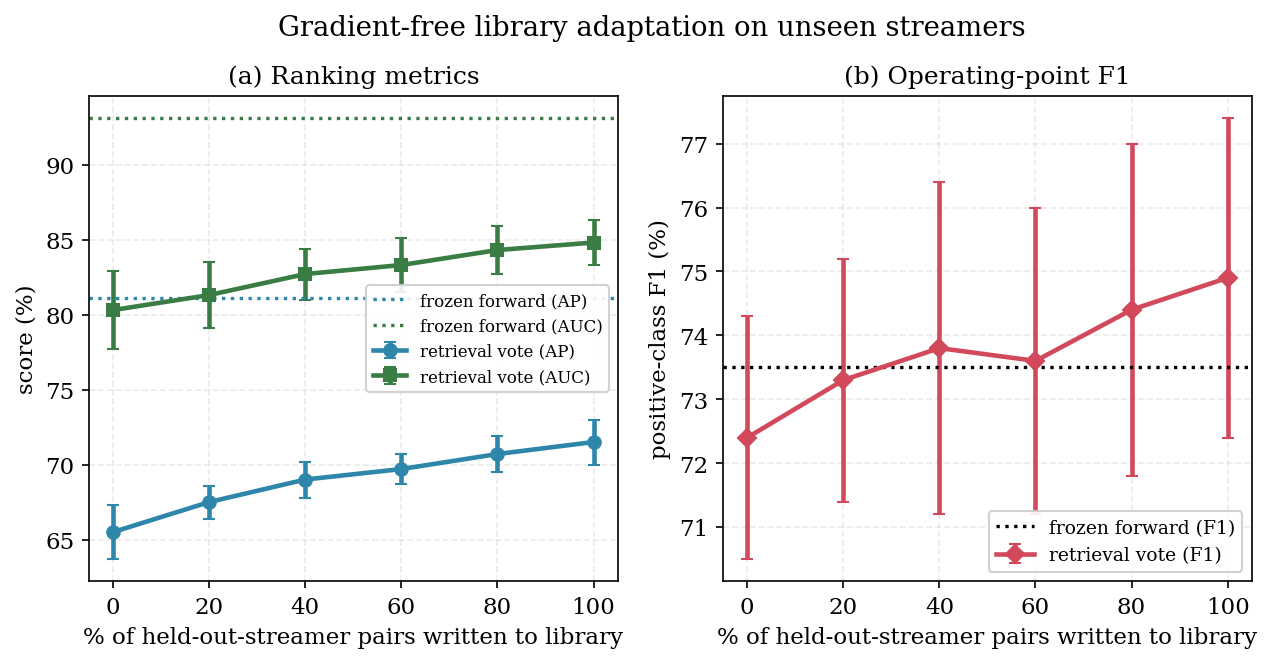
\includegraphics[width=\columnwidth]{figs/fig_inject.pdf}
\caption{Gradient-free library adaptation (leave-20-streamers). As held-out-streamer pairs enter the frozen-encoder library, the vote's AP and AUC climb toward the frozen forward classifier, showing new streamers are absorbed by index maintenance.}
\label{fig:inject}
\end{figure}

\subsection{Representation Geometry (RQ2)}

If the gain truly comes from the representation, it should be visible in the label geometry, so we hold the backbone, classifier, and hyper-parameters fixed and vary only the contrastive objective---no contrast (BCE only), standard SupCon \citep{khosla2020supcon}, and RACL (Table~\ref{tab:geom}). RACL produces the cleanest and most stable separation, lifting the label silhouette to 0.422 from SupCon's 0.349 and 0.196 without contrast. The comparison with SupCon is the more telling one: SupCon attains the tightest alignment but the weakest uniformity ($-0.86$), the signature of a partially collapsed space, whereas RACL keeps the embedding spread out ($-1.21$) while still pulling the classes apart---exactly the geometry that retrieval voting and library updates depend on. Both contrastive objectives raise hard-region purity@10 from 0.500 to 0.573, showing that the improvement is concentrated where it matters, among semantically close but oppositely labeled neighbors. The UMAP projection in Figure~\ref{fig:umap} makes the same point visually: the two classes interleave without contrast, SupCon tightens same-class clusters, and RACL detaches a clean high-risk cluster.

\begin{table}[t]
\centering\small
\setlength{\tabcolsep}{4pt}
\begin{tabular}{lcccc}
\toprule
Variant & Silh. & Hard pur.@10 & Align. & Unif. \\
\midrule
w/o contrast & 0.196\std{0.053} & 0.500\std{0.043} & 1.121 & $-2.02$ \\
SupCon & 0.349\std{0.173} & \best{0.573\std{0.017}} & \best{0.478} & $-0.86$ \\
\textbf{RACL} & \best{0.422\std{0.010}} & \best{0.573\std{0.088}} & 0.905 & $-1.21$ \\
\bottomrule
\end{tabular}
\caption{Label-conditional geometry of the test retrieval embedding under three contrastive objectives with an identical backbone (3-seed mean $\pm$ s.d.; metrics attribute-free).}
\label{tab:geom}
\end{table}

\begin{figure}[t]
\centering
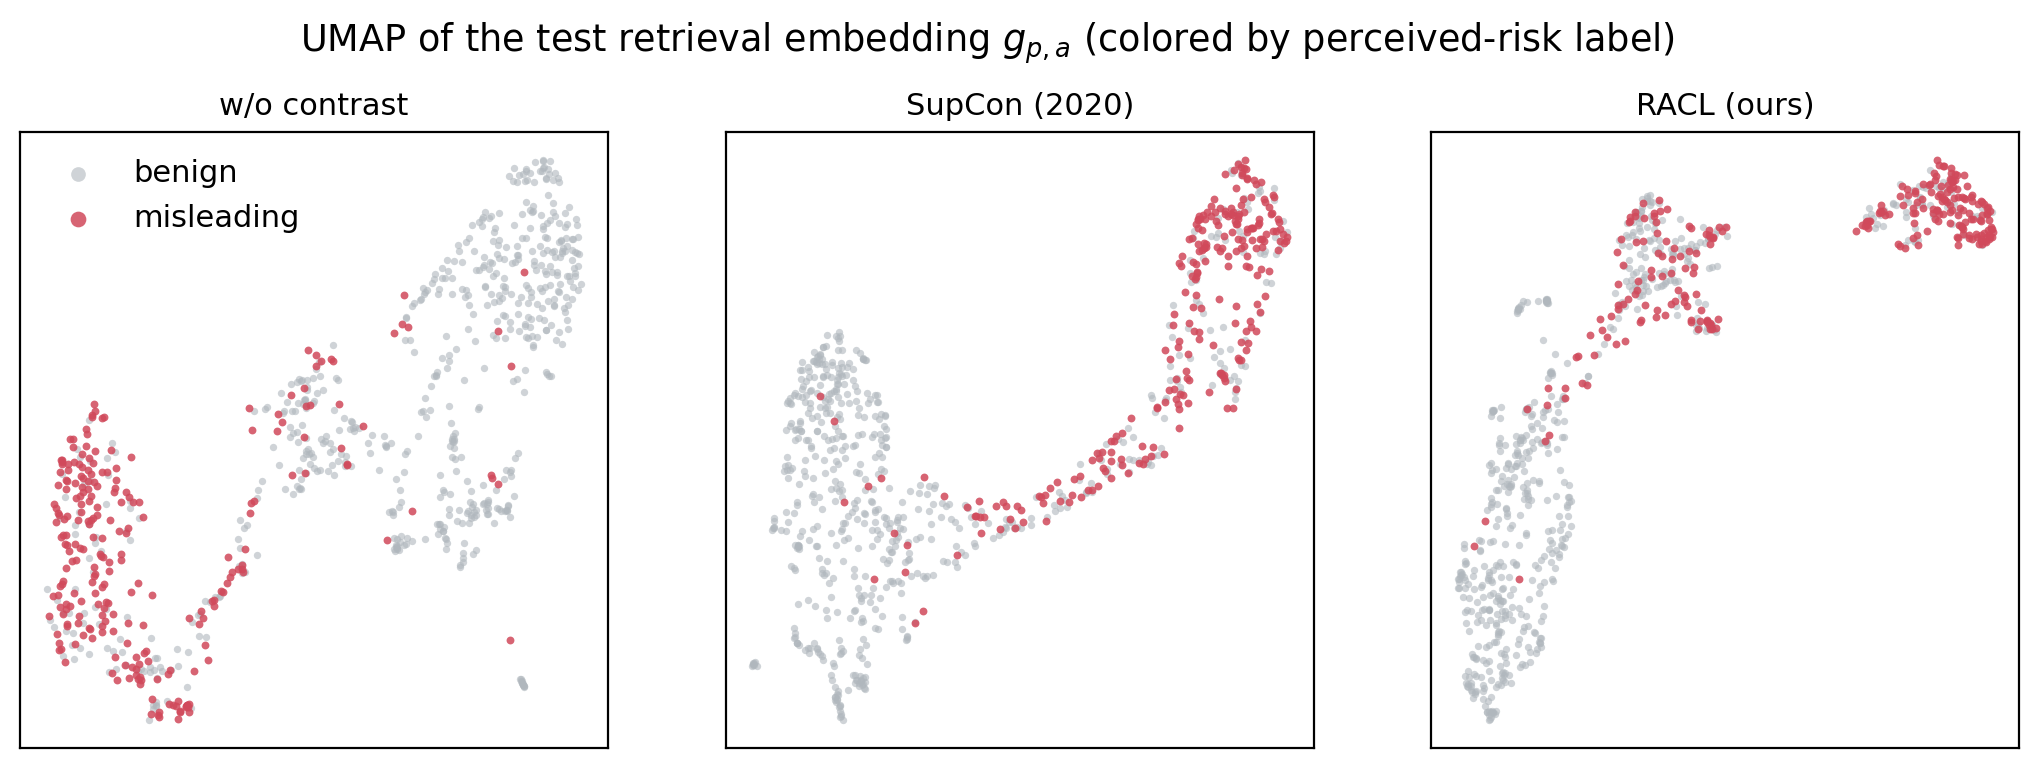
\includegraphics[width=\columnwidth]{figs/fig_umap_label.pdf}
\caption{UMAP of the test retrieval embedding $g_{p,a}$ colored by perceived-risk label (w/o contrast $\mid$ SupCon $\mid$ RACL). RACL isolates the misleading pairs into a detached cluster.}
\label{fig:umap}
\end{figure}

\subsection{Ablations (RQ4)}

To see which design choices carry the result, we change one at a time against the canonical configuration and always read the forward classifier, so the rows stay comparable. Three tables take up, in turn, the learning objective and backbone, the dual-stream architecture, and what the contrast retrieves.

\textbf{Objective, weighting, and backbone (Table~\ref{tab:abl_core}).} No single component is dispensable: every removal lowers both the operating point and the ranking metric. The contrastive objective and the reliability weight matter most, costing 3.3 and 3.2 AP respectively when dropped, which tells us that the learned geometry and the noise-aware supervision contribute roughly equally. The class-balancing factor adds a smaller but real 1.5 AP, and collapsing the ESIM four-tuple to a plain concatenation costs 3.6 AP, so the explicit difference and product features are not made redundant by fusion. Swapping the retrieval-pretrained BGE for BERT-base of similar size costs 4.3 AP---the single largest ranking drop---which places the gain in the backbone's retrieval pretraining rather than in raw capacity.

\textbf{Why two contrasting streams (Table~\ref{tab:abl_stream}).} The two streams play asymmetric but complementary roles. An evidence-only model collapses to 48.4 AP, barely above prevalence, because the product facts alone say nothing about whether a claim inflated expectations; a claim-only model fares better yet still gives up 5.0 AP, so the evidence stream does contribute once there is a claim to compare it against. Keeping both streams but removing the cross-attention fusion is the most damaging change to the operating point (4.6 F1), confirming that it is the cross-stream interaction---not mere access to both texts---that aligns a claim with its evidence. The streams and their interaction are therefore needed together.

\textbf{What to retrieve (Table~\ref{tab:abl_ret}).} Here the question is how to mine the contrastive examples, and two results stand out. Replacing pseudo-gold positives---the highest-similarity same-label neighbors---with conventional hard positives does not help and slightly lowers F1, mirroring the instability RGCL reports for hard positives \citep{mei2024rgcl}. Restricting the negatives, whether to the same attribute or the same evidence type, never beats the simpler class-balanced pool, so the canonical model keeps the latter. The number of positives is essentially inert ($K_p\in\{1,3,5\}$ all within noise), whereas the number of hard negatives has a clear optimum at five: too few (1.3 F1 lost) under-constrains the boundary, and too many (4.2 F1 lost) start importing noisy neighbors.

\begin{table}[t]
\centering\small
\setlength{\tabcolsep}{5pt}
\begin{tabular}{lcccc}
\toprule
Variant (forward) & Acc & F1 & AP & AUC \\
\midrule
\textbf{Canonical CLAIMARC} & \best{82.6}\std{0.4} & \best{73.4}\std{0.5} & \best{75.4}\std{1.3} & \best{90.4}\std{0.4} \\
w/o RACL contrast & 81.2\std{1.1} & 70.8\std{2.0} & 72.1\std{2.3} & 89.4\std{0.9} \\
w/o reliability weight & 81.6\std{1.3} & 71.6\std{1.6} & 72.2\std{3.1} & 89.5\std{0.7} \\
w/o class-balanced contrast & 82.1\std{0.5} & 72.7\std{1.9} & 73.9\std{0.4} & 89.9\std{0.2} \\
w/o ESIM four-tuple head & 81.4\std{0.6} & 72.0\std{1.7} & 71.8\std{2.3} & 89.4\std{0.5} \\
backbone: BGE $\to$ BERT & 81.2\std{0.6} & 72.4\std{0.9} & 71.1\std{1.4} & 89.2\std{0.4} \\
\bottomrule
\end{tabular}
\caption{Core objective, weighting, and backbone, removed one at a time (\%, forward classifier, 3-seed mean $\pm$ s.d.).}
\label{tab:abl_core}
\end{table}

\begin{table}[t]
\centering\small
\setlength{\tabcolsep}{5pt}
\begin{tabular}{lcccc}
\toprule
Stream design & Acc & F1 & AP & AUC \\
\midrule
\textbf{Dual + TwoStreamFusion} & \best{82.6}\std{0.4} & \best{73.4}\std{0.5} & \best{75.4}\std{1.3} & \best{90.4}\std{0.4} \\
Dual, w/o fusion (concat) & 80.7\std{0.5} & 68.8\std{3.2} & 73.8\std{1.4} & 89.6\std{0.4} \\
Claim stream only & 81.1\std{1.0} & 73.0\std{0.3} & 70.4\std{1.9} & 89.2\std{0.1} \\
Evidence stream only & 68.7\std{0.8} & 44.1\std{4.3} & 48.4\std{0.4} & 68.7\std{1.2} \\
\bottomrule
\end{tabular}
\caption{Necessity of two contrasting streams (\%, forward classifier, 3-seed mean $\pm$ s.d.).}
\label{tab:abl_stream}
\end{table}

\begin{table}[t]
\centering\small
\setlength{\tabcolsep}{5pt}
\begin{tabular}{lcccc}
\toprule
RACL retrieval design & Acc & F1 & AP & AUC \\
\midrule
\textbf{Pseudo-gold pos., global} & \best{82.6}\std{0.4} & \best{73.4}\std{0.5} & \best{75.4}\std{1.3} & \best{90.4}\std{0.4} \\
\ \ hard neg. ($K_p3/K_n5$) & & & & \\
hard positives (vs.\ pseudo-gold) & 81.9\std{1.1} & 73.0\std{0.7} & 73.7\std{0.7} & 90.0\std{0.2} \\
same-attribute negatives & 82.1\std{0.4} & 72.6\std{1.3} & 73.5\std{0.5} & 90.0\std{0.0} \\
same-evidence-type negatives & 81.8\std{0.3} & 72.7\std{1.5} & 74.0\std{0.5} & 90.0\std{0.1} \\
positives $K_p{=}1$ & 82.5\std{0.7} & 73.4\std{0.6} & 74.0\std{0.7} & 89.9\std{0.2} \\
hard negatives $K_n{=}1$ & 81.4\std{0.4} & 72.1\std{1.4} & 73.6\std{0.2} & 90.0\std{0.1} \\
hard negatives $K_n{=}10$ & 81.1\std{0.3} & 69.2\std{2.3} & 73.5\std{0.4} & 89.9\std{0.1} \\
\bottomrule
\end{tabular}
\caption{Retrieval-augmented contrast: positive/negative mining (\%, forward classifier, 3-seed mean $\pm$ s.d.). Restricting negatives never helps.}
\label{tab:abl_ret}
\end{table}

\textbf{Is the reliability weight well constructed?} Since $c_{p,a}$ moves the headline numbers, a fair question is whether its particular form is necessary or whether any down-weighting of low-signal samples would do. To answer it we perturb only the per-sample \emph{training} weight $w_{p,a}$, leaving the architecture, data, and the validation/test weights untouched so that thresholds and weighted metrics remain comparable (Table~\ref{tab:rw}). The perturbations isolate three properties of the design. Its direction is informative: removing the weight costs 2.2 F1, and reversing it---trusting exactly the samples the design judges least reliable---costs 5.7 F1 and drops below the uniform baseline. Its assignment, not its marginal shape, is what helps: permuting $c$ across pairs returns to the uniform level. And its continuity is what protects the ranking: coarsening $c$ to a median split is the harshest change of all ($-7.0$ AP), so a graded weight, rather than a reliable/unreliable switch, preserves the precision--recall ordering. The composite form also earns its keep---reducing it to the saturation term alone costs 1.5 F1, so the asymmetric-diagnosticity and authenticity factors add information beyond a simple review count. The only harmless edit is an order-preserving square-root reshaping, which confirms that the design tolerates how steeply samples are graded but not reversing, flattening, or shuffling that grading.

\begin{table}[t]
\centering\small
\setlength{\tabcolsep}{5pt}
\begin{tabular}{lcccc}
\toprule
Training weight $w$ & Acc & F1 & AP & AUC \\
\midrule
\textbf{Canonical} ($w{=}c$) & \best{82.6}\std{0.4} & 73.4\std{0.5} & \best{75.4}\std{1.3} & \best{90.4}\std{0.4} \\
Uniform ($w{=}1$) & 81.6\std{1.2} & 71.2\std{1.6} & 73.3\std{2.3} & 89.6\std{0.6} \\
Reversed & 80.0\std{0.4} & 67.7\std{3.5} & 74.1\std{1.9} & 89.5\std{0.3} \\
Permuted across pairs & 80.4\std{0.6} & 71.6\std{1.5} & 73.0\std{2.8} & 89.4\std{0.8} \\
Median-split (binary) & 79.5\std{0.8} & 70.2\std{2.5} & 68.4\std{1.1} & 88.3\std{0.7} \\
Saturation term only & 80.3\std{0.3} & 71.9\std{0.4} & 73.1\std{1.6} & 89.1\std{0.4} \\
Square-root ($w{=}\sqrt c$) & 81.8\std{1.5} & \best{74.0}\std{1.3} & 72.6\std{2.5} & 89.9\std{0.5} \\
\bottomrule
\end{tabular}
\caption{Counterfactual reliability weightings (\%, forward classifier, 3-seed mean $\pm$ s.d.). Only the per-sample training weight is altered. The canonical $w{=}c$ is best on Accuracy, AP, and AUC.}
\label{tab:rw}
\end{table}

\subsection{Selective Prediction and Error Analysis}

In practice the model runs in front of human reviewers, so part of its value is knowing when to defer. The forward classifier and the RKC vote are two near-independent readings of the same pair, and their disagreement $|\hat y_t-\hat y^{\mathrm{RKC}}_t|$ gives a training-free gate for abstention. Routing the highest-disagreement pairs to human review steadily improves what the model decides on its own: cutting coverage to 80\% lifts accuracy from 0.814 to 0.867 and selective AP from 0.737 to 0.778, and the trend continues to 0.889 accuracy at 70\% and 0.908 at 65\%. The gate is doing more than shrinking the set---a random abstention of the same size leaves accuracy and AP essentially flat ($\approx0.81$ and $\approx0.73$), so disagreement genuinely localizes the hard cases (Figure~\ref{fig:selective}). A single temperature scale further pulls the predicted probabilities onto the diagonal (Figure~\ref{fig:calib}), which is what a decision-support tool needs.

The errors that remain are interpretable and point to a clear bottleneck. At the validation-selected operating point CLAIMARC recalls 84\% of misleading pairs (TP$=$210, FN$=$39) at FP$=$120, the recall-favoring trade-off a screening tool should make, and its error rate falls as more evidence is available (24.1\% / 16.4\% / 10.3\% for one, two, and three sources), so the residual limit is evidence acquisition rather than the discriminator. Two failure modes recur. False negatives are mostly terse stylized endorsements (``fleece-lined,'' ``the texture is really top-tier'') that buyers later read as misleading despite no surface contradiction---precisely the sparse-signal cases that objective verification and LLMs also miss. False positives cluster on vivid but harmless figures of speech (``it goes on like a coating'' for a foam product), where the model over-reads risk. Notably, CLAIMARC and a fine-tuned BERT err on largely different pairs---each fixes about 44 of the other's mistakes and only 114 are wrong for both---which points to a retrieval-augmented ensemble of complementary encoders as a natural next step.

\begin{figure}[t]
\centering
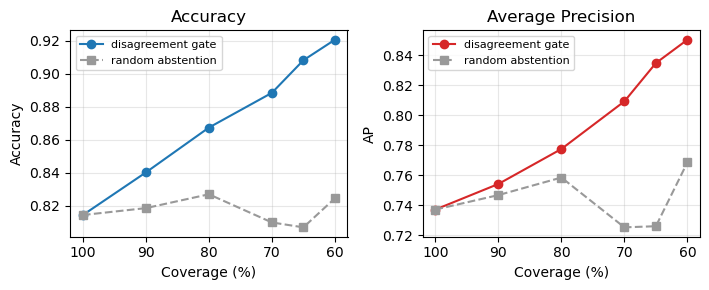
\includegraphics[width=\columnwidth]{figs/fig_selective.pdf}
\caption{Selective prediction. Abstaining on the highest forward-RKC disagreement and routing those pairs to human review improves selective AP and accuracy on the remainder, whereas a random abstention of the same size (dashed) stays flat.}
\label{fig:selective}
\end{figure}

\begin{figure}[t]
\centering
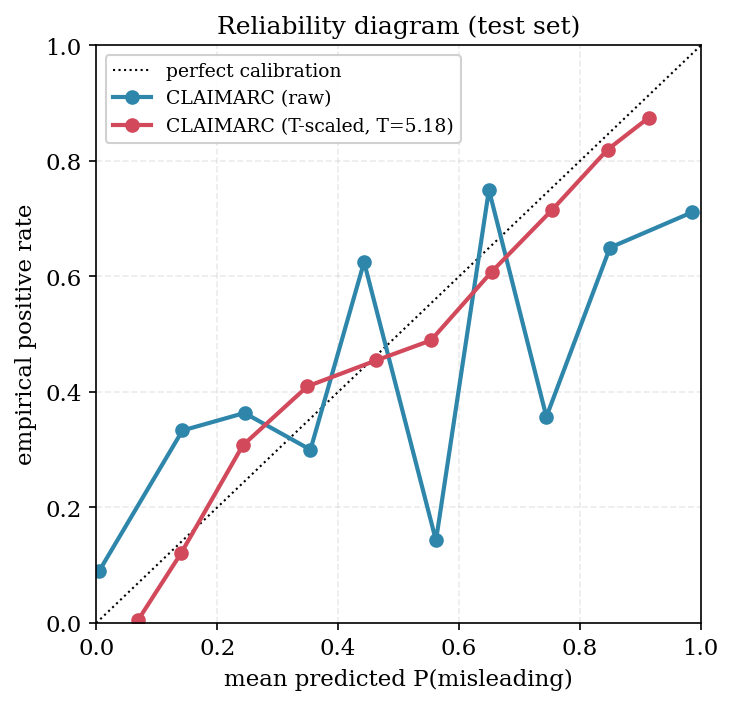
\includegraphics[width=0.78\columnwidth]{figs/fig_calibration.pdf}
\caption{Reliability diagram (test). A single temperature scale brings CLAIMARC's predicted probabilities close to the diagonal.}
\label{fig:calib}
\end{figure}

\subsection{Hyper-parameter Sensitivity and Efficiency}

A method is easier to trust if its result does not hinge on careful tuning, so we sweep the five knobs most likely to matter---fusion depth $N$, attention heads, retrieval-head dimension, temperature $\tau$, and the retrieval sizes $(K_p,K_n)$. AP stays inside a narrow 0.69--0.74 band throughout, with the canonical setting on the flat part of every curve; the one exception is an oversized retrieval set $(5,10)$, which degrades by pulling in noisy neighbors (Figure~\ref{fig:hparam}). The full single-seed sweep, along with the loss-function, feed-forward, cross-attention-direction, projection-sharing, and evidence-composition variants, is deferred to the appendix (Table~\ref{tab:sweep}), which also examines the reliability-weight formula itself (Table~\ref{tab:rwformula}). For deployment at lower cost, a parameter-efficient variant that freezes the backbone and trains only LoRA adapters and the new modules gives up about 5 AP while still supporting gradient-free library writes, covering the maintenance end of the spectrum.

\begin{figure}[t]
\centering
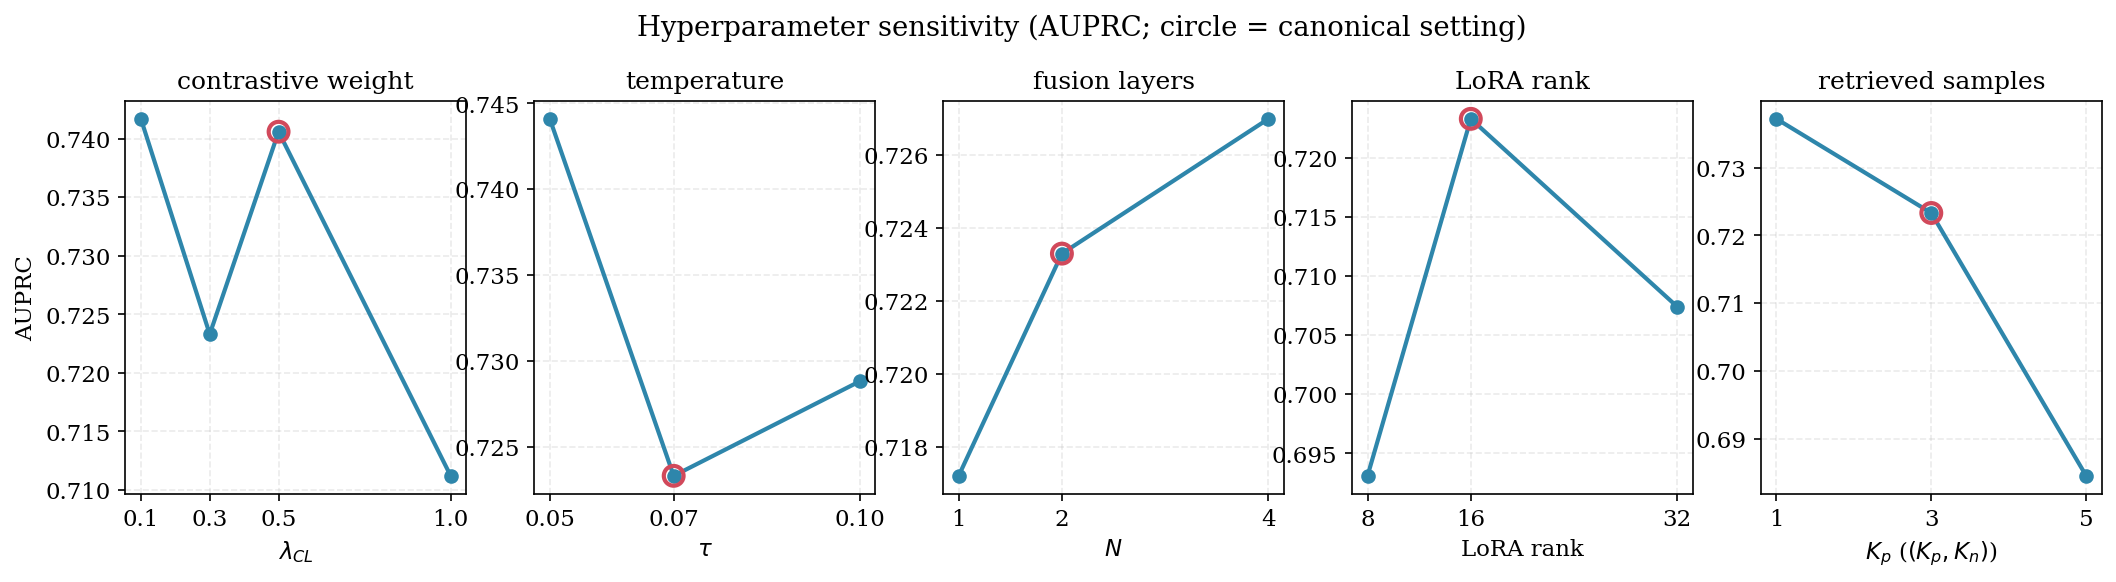
\includegraphics[width=\columnwidth]{figs/fig_hparam.pdf}
\caption{Hyper-parameter sensitivity (AP). Across all five sweeps the score stays in a narrow band; the canonical configuration (circled) sits on the stable plateau.}
\label{fig:hparam}
\end{figure}

\section{Conclusion}

CLAIMARC treats livestream misleading-advertising detection as attribute-level consumer-perception discrimination rather than fact verification. The reframing holds up empirically: objective verification and zero-shot LLMs miss the label, whereas a dual-stream encoder trained with reliability-weighted retrieval-augmented contrast ranks better, learns a cleaner representation, and transfers further. Controlled analyses trace the gain to the learned representation rather than the retrieval rule, and show that the fixed encoder absorbs new streamers by maintaining its index while a classifier--retrieval disagreement gate turns the model into a calibrated triage front end. Residual errors concentrate in terse endorsements and thin-evidence cases, pointing toward richer evidence acquisition and an ensemble of complementary encoders.

\bibliography{claimarc_refs}

\appendix
\section{Appendix: Extended Sweeps}

Table~\ref{tab:sweep} reports the full single-seed hyper-parameter and variant sweep summarized in the main text, spanning model capacity (fusion depth, heads, LoRA rank), the contrastive objective ($\lambda_{\mathrm{CL}}$, $\tau$, retrieval sizes, loss), architecture (feed-forward activation, cross-attention direction, projection sharing), and evidence composition. To control sweep cost these runs use the parameter-efficient LoRA-frozen variant; every row reads the forward classifier on the test set, with the canonical configuration in bold. The five core knobs keep AP within a 0.69--0.74 band; single-source evidence policies reach high peak AP on individual views but the canonical mix is kept for coverage when a given view is sparse.

\begin{table}[t]
\centering\small
\setlength{\tabcolsep}{5pt}
\begin{tabular}{lcccc}
\toprule
Configuration & Acc & F1 & AP & AUC \\
\midrule
\textbf{Canonical} ($N2,h8,r16,$ & \best{82.6} & \best{73.4} & \best{75.4} & \best{90.4} \\
\ \ $\lambda.5,\tau.07,K35$) & & & & \\
\multicolumn{5}{l}{\emph{Fusion blocks $N$}} \\
$N{=}1$ & 80.9 & 72.1 & 72.7 & 89.2 \\
$N{=}3$ & 80.6 & 72.6 & 72.6 & 89.5 \\
$N{=}4$ & 80.2 & 70.8 & 70.0 & 86.9 \\
\multicolumn{5}{l}{\emph{Attention heads}} \\
4 heads & 80.5 & 70.0 & 71.0 & 89.0 \\
16 heads & 79.9 & 70.9 & 70.5 & 88.9 \\
\multicolumn{5}{l}{\emph{LoRA rank}} \\
rank 8 & 80.6 & 71.8 & 70.5 & 89.1 \\
rank 32 & 81.0 & 73.3 & 73.6 & 89.6 \\
\multicolumn{5}{l}{\emph{Contrastive weight $\lambda_{\mathrm{CL}}$}} \\
0.1 / 0.3 / 1.0 & 79.8 & 70.8 & 69.8 & 88.0 \\
\multicolumn{5}{l}{\emph{Temperature $\tau$}} \\
0.05 / 0.10 / 0.20 & 80.0 & 70.6 & 69.5 & 88.2 \\
\multicolumn{5}{l}{\emph{Retrieval sizes $(K_p,K_n)$}} \\
(1,1) & 79.8 & 70.9 & 70.0 & 88.1 \\
(5,10) & 80.0 & 70.4 & 69.5 & 87.9 \\
\multicolumn{5}{l}{\emph{Loss function}} \\
ASL & 81.3 & 72.7 & 71.8 & 88.8 \\
Focal & 79.9 & 68.7 & 68.6 & 87.4 \\
\multicolumn{5}{l}{\emph{Architecture}} \\
FFN GeLU (vs.\ SwiGLU) & 80.0 & 69.7 & 71.7 & 88.7 \\
cross-attn.\ claim$\to$ev. & 81.4 & 69.7 & 71.2 & 88.1 \\
cross-attn.\ ev.$\to$claim & 80.3 & 72.4 & 68.0 & 88.3 \\
independent projections & 81.3 & 72.8 & 73.6 & 89.8 \\
\multicolumn{5}{l}{\emph{Evidence policy}} \\
params only & 82.0 & 72.4 & 74.1 & 89.8 \\
OCR only & 80.3 & 68.5 & 75.2 & 89.4 \\
VLM only & 81.3 & 73.8 & 75.6 & 90.0 \\
\bottomrule
\end{tabular}
\caption{Single-seed hyper-parameter and variant sweep (\%, forward classifier, test set; LoRA-frozen variant).}
\label{tab:sweep}
\end{table}

\begin{table}[t]
\centering\small
\setlength{\tabcolsep}{5pt}
\begin{tabular}{llcccc}
\toprule
Parameter & Set & Acc & F1 & AP & AUC \\
\midrule
\textbf{Canonical} & --- & \best{82.6} & \best{73.4} & \best{75.4} & \best{90.4} \\
Saturation $k$ & 1.5 & 78.7 & 72.4 & 72.6 & 89.3 \\
 & 6.0 & 79.0 & 63.9 & 67.8 & 88.1 \\
Asym.\ disc.\ $\lambda$ & 0.1 & 81.2 & 73.9 & 71.6 & 89.5 \\
 & 0.6 & 80.5 & 68.8 & 72.3 & 89.1 \\
Fake disc.\ $\rho$ & 0.2 & 81.8 & 70.7 & 72.1 & 89.5 \\
 & 0.6 & 80.9 & 70.4 & 70.0 & 88.8 \\
Strong-neg $\phi$ & 1.0 & 78.6 & 72.0 & 68.8 & 88.7 \\
 & 1.5 & 81.6 & 70.8 & 71.2 & 89.2 \\
\bottomrule
\end{tabular}
\caption{Reliability-weight formula sensitivity (\%, forward classifier, test set). One hyper-parameter of the $c$ construction is moved at a time and $c$ is recomputed (single seed; canonical is the 3-seed reference). Every excursion lowers AP, with the saturation rate $k$ and the strong-negative bonus $\phi$ the most sensitive.}
\label{tab:rwformula}
\end{table}

\section*{Reproducibility Checklist}

\textbf{General.} This paper includes a conceptual description of the proposed method, including the data unit, model architecture, the retrieval-augmented contrastive objective, and the inference procedure. Objective results are separated from interpretation, and background work is cited for fact verification, consumer-perception risk, contrastive representation learning, and dense retrieval.

\textbf{Theoretical contributions.} This paper does not make formal theoretical contributions; its claims are empirical.

\textbf{Datasets.} The experiments use a newly constructed Chinese livestream e-commerce dataset, motivated by the need to study consumer-perceived misleading advertising where objective contradiction labels are insufficient. The construction pipeline, annotation target, label reliability, attribute-level unit, and room-grouped split are described in the paper. Public release depends on platform and privacy constraints; at minimum, anonymized preprocessing scripts, split files, and derived feature/label metadata sufficient to reproduce the reported experiments will be submitted where platform terms permit redistribution.

\textbf{Computational experiments.} The paper states the evaluation metrics, reports mean and standard deviation over three random seeds, and uses paired bootstrap intervals. The split is grouped by room ID to prevent streamer leakage; the validation set selects thresholds for Accuracy and F1, while AP and AUC are threshold-free. All trainable baselines and CLAIMARC use seeds 0, 1, and 2. The canonical CLAIMARC fully fine-tunes BGE-large-zh-v1.5; the parameter-efficient variant freezes BGE and trains LoRA adapters, LayerNorm parameters, special-token embeddings, the fusion module, and heads for deployment analysis only. Final hyper-parameters include 3 classification-only warm-up epochs, 6 RACL epochs, $K_p{=}3$, $K_n{=}5$, $\tau{=}0.07$, $\lambda_{\mathrm{CL}}{=}0.5$, and a 256-dimensional retrieval head. Anonymized supplementary code for preprocessing, training, evaluation, ablation, and figure generation will be submitted.

\end{document}
